% TO-DO:  Kolmogorov complexity

\documentclass[17pt]{beamer}
\usepackage[CJKspace]{xeCJK}
%\usepackage{newtxtext,newtxmath}	% use Times Roman font
%\usefonttheme{serif}
\usefonttheme{professionalfonts}
%\setbeamertemplate{theorems}[numbered]
\setbeamertemplate{caption}{\insertcaption} 	% no `Figure' prefix before caption

\mode<presentation> {

%\usetheme{default}
%\usetheme{AnnArbor}
%\usetheme{Antibes}
%\usetheme{Bergen}
%\usetheme{Berkeley}
%\usetheme{Berlin}
%\usetheme{Boadilla}
%\usetheme{CambridgeUS}
%\usetheme{Copenhagen}
%\usetheme{Darmstadt}
%\usetheme{Dresden}
%\usetheme{Frankfurt}
%\usetheme{Goettingen}
%\usetheme{Hannover}
%\usetheme{Ilmenau}
%\usetheme{JuanLesPins}
%\usetheme{Luebeck}
\usetheme{Madrid}
%\usetheme{Malmoe}
%\usetheme{Marburg}
%\usetheme{Montpellier}
%\usetheme{PaloAlto}
%\usetheme{Pittsburgh}
%\usetheme{Rochester}
%\usetheme{Singapore}
%\usetheme{Szeged}
%\usetheme{Warsaw}

%\usecolortheme{albatross}
%\usecolortheme{beaver}
%\usecolortheme{beetle}
%\usecolortheme{crane}
%\usecolortheme{dolphin}
%\usecolortheme{dove}
%\usecolortheme{fly}
%\usecolortheme{lily}
%\usecolortheme{orchid}
%\usecolortheme{rose}
%\usecolortheme{seagull}
%\usecolortheme{seahorse}
%\usecolortheme{whale}
%\usecolortheme{wolverine}

%\setbeamertemplate{footline} % To remove the footer line in all slides uncomment this line
%\setbeamertemplate{footline}[page number] % To replace the footer line in all slides with a simple slide count uncomment this line
\setbeamertemplate{navigation symbols}{} % To remove the navigation symbols from the bottom of all slides uncomment this line
}

\renewcommand\textbullet{\leavevmode%
	\usebeamertemplate{itemize item}\hspace{.5em}}

\usepackage{graphicx} % Allows including images
\usepackage{verbatim} % comments
% \usepackage{tikz-cd}  % commutative diagrams
% \newcommand{\tikzmark}[1]{\tikz[overlay,remember picture] \node (#1) {};}
% \usepackage{booktabs} % Allows the use of \toprule, \midrule and \bottomrule in tables
% \usepackage{amssymb}  % \leftrightharpoons
\usepackage{wasysym} % frownie face

\newcommand{\vect}[1]{\boldsymbol{#1}}
\newcommand*\sigmoid{\vcenter{\hbox{
\includegraphics{sigmoid.png}}}}

\makeatletter
\renewcommand{\boxed}[1]{\fbox{\m@th$\displaystyle\scalebox{0.9}{#1}$} \,}
\makeatother

%---------------------------- make slide margin narrower --------------------------------
\newcommand\Wider[2][3em]{%
	\makebox[\linewidth][c]{%
		\begin{minipage}{\dimexpr\textwidth+#1\relax}
			\raggedright#2
		\end{minipage}%
}%
}

%----------------------------------------------------------------------------------------
%	TITLE PAGE
%----------------------------------------------------------------------------------------

\title[Logic AI]{{\normalsize 不要再怪我没教你:}\\ Logic-based AI 入门} % The short title appears at the bottom of every slide, the full title is only on the title page

\author{YKY 甄景贤} % Your name
\institute[] % Your institution as it will appear on the bottom of every slide, may be shorthand to save space
{
Independent researcher, Hong Kong \\ % Your institution for the title page
\medskip
\textit{generic.intelligence@gmail.com} % Your email address
}
\date{\today} % Date, can be changed to a custom date

\begin{document}

\frame{\titlepage}

\begin{frame}
\frametitle{Talk summary}
\tableofcontents
\end{frame}

%---------------- this is for when you're using \part's ----------------------------------
%\begin{frame}
%\frametitle{Summary}
%
%{\usebeamerfont*{frametitle} Part I %\usebeamercolor[fg]{frametitle}
% ~ ~ ~ Deep reinforcement learning}
%%\tableofcontents[part=1]
%
%\vspace{1.5cm}
%{\usebeamerfont*{frametitle} Part II %\usebeamercolor[fg]{frametitle}
% ~ ~ ~ Logical structure}
%%\tableofcontents[part=2]
%\end{frame}

%----------------------------------------------------------------------------------------
%	PRESENTATION SLIDES
%----------------------------------------------------------------------------------------

%------------------------------------------------

%\part{title}

% \fontsize{16}{15}\selectfont

\begin{frame}
\frametitle{为什么要学 logic-based AI?}
\begin{itemize}
	\item \textbf{神经网络/深度学习} 是现时 (2019) 最强的学习算法
	\item 某种意义上说,逻辑 AI 已经过时
	\item 很多人(包括外国)不熟悉 逻辑 AI,所以看不懂我的 理论,还有 OpenCog、OpenNARS 这些「第一代」AGI
	\item 逻辑 是 强人工智能 的基础
\end{itemize}
\end{frame}

\section[Section]
{\texorpdfstring{逻辑 是 什么?}
	{逻辑 是 什么?}}
\frame{\sectionpage}

\begin{frame}
\frametitle{历史: Aristotle (ca. 300BC)}
\textbullet 逻辑学 研究 (人类) 思考的方式
\fontsize{16}{16}\selectfont
\begin{minipage}[t]{0.48\linewidth}
	\begin{itemize}
		\item 亚里士多德 \\
			三段论 (syllogism)
		\item 例: \\
			所有人都会死 \\
			苏格拉底 是人 \\
			苏格拉底 会死
	\end{itemize}
\end{minipage}
\hfill
\begin{minipage}[t]{0.48\linewidth}
	\begin{figure}[H]
		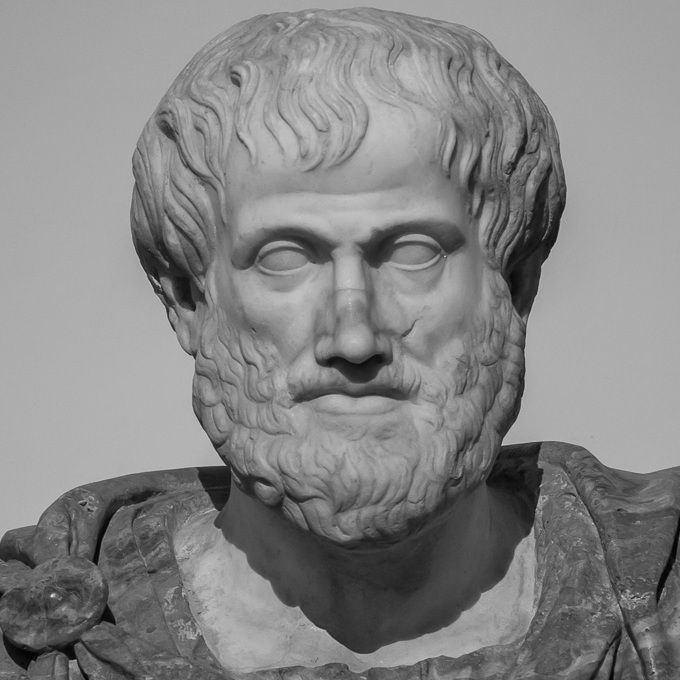
\includegraphics[scale=0.25]{Aristotle.jpg}
	\end{figure}
\end{minipage}
\end{frame}

\begin{frame}
\frametitle{\large 有没有 不能用 逻辑 表达的思想?}
\begin{itemize}
	\item 如果有,你必须把它用文字表述出来
	\item 基本上,任何语言表述 可以 转化成 逻辑形式
	\item 所以,一定讲不出来
\end{itemize}
\end{frame}

\section[Section]{逻辑的种类}
\frame{\sectionpage}

\begin{frame}
\frametitle{范畴 逻辑 (categorical logic)}
\begin{itemize}
	\item blah
\end{itemize}
\end{frame}


\section[Section]{逻辑 AI 的 系统架构}
\frame{\sectionpage}

\section[Section]{推导 算法}
\frame{\sectionpage}

\section[Section]{概率/模糊 逻辑}
\frame{\sectionpage}

\section[Section]{学习算法}
\frame{\sectionpage}

\section*{结论}

\begin{frame}
\frametitle{中国}
\Wider[1em]{
\begin{itemize}
	\item AGI 项目
\end{itemize}
}
	\begin{center}
		多谢收看 \smiley{}
	\end{center}
\end{frame}

\begin{comment}

\begin{frame}
\frametitle{References}
\footnotesize{
\begin{thebibliography}{99} % Beamer does not support BibTeX so references must be inserted manually as below
\bibitem[]{} Bart Jacobs (1999)
\newblock Categorical logic and type theory
% \newblock \emph{North Holland, Studies in logic} v141.

\bibitem[]{} Robert Goldblatt (2006)
\newblock Topoi -- the categorical analysis of logic

\end{thebibliography}
}
\end{frame}

\begin{frame}
We're looking for developers to implement a prototype.

\vspace*{1cm}
\Large{\centerline{Thank you}}

%\vspace*{1cm}
%\Large{\centerline{The End}}
\end{frame}

\end{comment}

\end{document} 